\section*{Ménard e Shirley (2014): The future of new institutional economics: from early intuitions to a new paradigm?}

\subsection*{Introdução}


Os autores destacam a NEI tem apresentado um notório crescimento e relevância nos últimos 20 anos e que o diálogo entre as diferentes variantes da NEI tem aumentado com a criação da ISNIE. Pontuam que apesar dessas discussões, a NEI continua sendo  uma área descentralizada, de modo que não há uma teórica geral das instituições. Em linhas gerais, é caracterizada pela ênfase nas instituições como \textbf{normas e regras}, na microanálise das formas de organização (firmas e mercados) de forma multidisciplinar por meio de, em grande medida, estudos de casos.

\subsection*{Origens intelectuais da NEI}

\subsubsection*{Influências}

Ao longo desta seção, Ménard e Shirley traçam as principais influências da NEI e suas correntes dominantes.

\subsubsection*{Conceitos principais}

Em conjunto com as hipóteses comportamentais, a NEI possui três conceitos principais:

\begin{description}
	\item[Custos de transação:] Este conceito é importante para NEI porque é relevante para o sistema econômico uma vez que a forma de se organizar as transações determina o que é produzido e a capacidade de desfrutar da divisão do trabalho;
	\item[Direitos de propriedade:] A designação dos direitos de propriedade se torna mais importante na presença de custos de transação. Além disso, Coase destaca que uma transação é, no limite, transação de direitos de tomar ações. Williamson pontuou que os direitos de propriedade estão sujeitos às consequências negativas do comportamento oportunista e que os custos de se recorrer a judicialização são maiores do que os acordos privados.
	\item[Contratos:] Assim como os demais conceitos, Coase é o responsável pela introdução dos contratos na NEI. Em linhas gerais, tal inclusão se destoa do modelo usual por
	\begin{itemize}
		\item Não são perfeitamente executados
		\item Serem incompletos
	\end{itemize}
	Williamson, em especial, analisa os tipos de contratos de acordo com os seguintes atributos:
	\begin{itemize}
		\item Preço
		\item Salvaguardas
		\item Especificidade dos ativos envolvidos
	\end{itemize}
\end{description}

\subsection*{Das ideias preliminares ao instrumental analítico}

A partir das contribuições de Coase, surgiram duas principais bifurcações na NEI: Willianson e North

\begin{figure}[h]
	\centering
	\caption{Influências da NEI}
	\label{fig:screenshot001}
	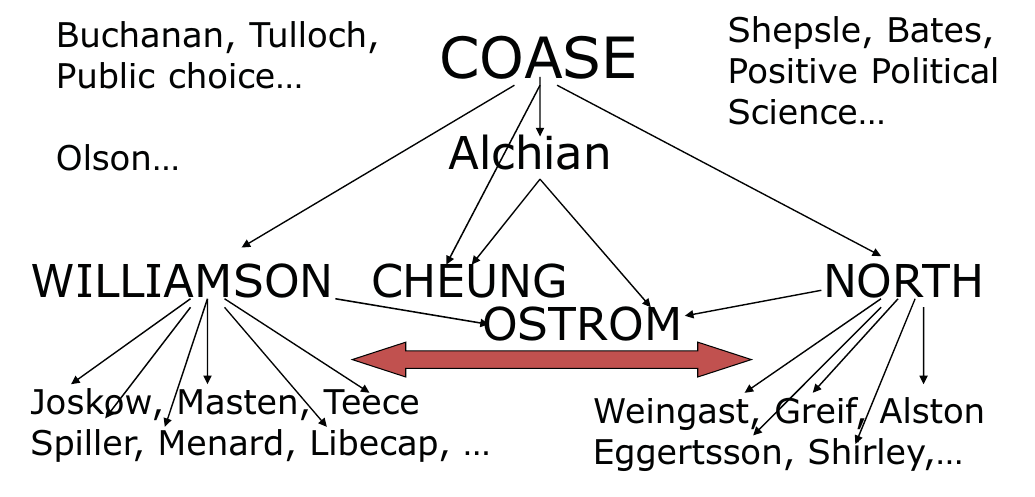
\includegraphics[width=0.7\linewidth]{screenshot001}
\end{figure}


\subsubsection*{Williamson e os custos de transação}

Dentre os temas investigados por Williamson, destaca-se:

\begin{itemize}
	\item Incentivos, controle e gestão;
	\item Grupos pequenos, complexidade e incerteza
	\item Atributos dos contratos
	\begin{itemize}
		\item Incerteza
		\item Frequência
		\item Especificidade
	\end{itemize}
	\item Verticalização e formas de organização
	\item Regulação e estruturas de governança
\end{itemize}


\subsubsection*{North e a análise institucional}

North partiu de uma análise institucional para explicar o desenvolvimento econômico ocidental, destacando contratos formais e --- posteriormente --- regime político, ideologia e crenças. Em linhas gerais, ao avaliar os determinantes da \textbf{mudança institucional}, North conclui que endogenamente no ``mercado político''. Em seguida, debruçou-se sobre ciências cognitivas e aprendizado .

\subsection*{Difusão e sucesso da NEI}

Ao longo desta seção, o autores apresentam dados que evidenciam o repentino e crescente interesse nos temas da NEI. Dentre os fatores que contribuíram para esse maior interesse, destaca-se a criação da ISNEI e colapso das economias planejadas e subsequentes discussões a configuração destes novos sistemas econômicos emergentes.
Além disso, os autores destacam a incorporação de instituições nos moldes neoclássicos ao longo dos anos 90.


\subsection*{O futuro da NEI}

Os autores colocam a seguinte questão: seria a NEI uma alternativa ou um complemento ao paradigma dominante? De todo modo, concluem que o conceito de custos de transação não pode ser desassociado do porquê da existência das firmas. Além disso, por conta dos custos de transação, os direitos de propriedade não podem ser definidos perfeitamente, ou os contratos não podem ser perfeitamente elaborados e implementados dado o comportamento oportunista (\textit{ex post}). Em outras palavras, custos de transação implicam que instituições devem ser analisadas. 
Destacam também que a NEI têm incorporado modelos mentais compartilhados e considerado estruturas de organização híbridas.
Adiante, os autores pontuas as dificuldades metodológicas para se construir uma teoria das instituições.
Dentre as dificuldades, destaca-se a ausência de consenso na definição de instituições que extrapola as variantes teóricas (Williamsonians e Northianas). Em resumo, as dificuldades são (p.~559):

\begin{quotation}
	Besides developing a more robust theory, NIE faces a number of other
	challenges if it is to flesh out a convincing paradigm. These include: overcoming
	the internal divisions mentioned above; dealing more deeply with institutional
	change; expanding the empirical and theoretical work on informal institutions;
	developing data to allow more careful definition and measurement of the
	effects of institutions in a variety of settings; building more adequate models
	to capture the links between theory and empirical analyses.
\end{quotation}

Em seguida, destacam o progresso da NEI a partir de \textbf{estudos de caso} em que vale destacar a seguinte passagem (p.~560):

\begin{quotation}
	Despite the poor opinion that most mainstream economists have of case studies,
	they have proven to be a valuable tool for understanding the rich details
	inherent in institutional analysis, especially when they are informed by theory
	and conducted with rigor.
	
\end{quotation}

\subsubsection*{Conclusão}

Os autores são otimistas em relação à difusão da NEI no futuro em grande medida por seu caráter multidisciplinar e interesse de acadêmicos dos países em desenvolvimento. Finalizam pontuam a importância de Coase.

	\begin{sigstatement}
			\sffamily
			\mdfdefinestyle{stylesigstyle}{linewidth=0.7pt,
				backgroundcolor=styleblueback,linecolor=stylebluetext,
				fontcolor=stylebluetext,innertopmargin=6pt,innerrightmargin=6pt,
				innerbottommargin=6pt,innerleftmargin=6pt}
			{%	
				\begin{mdframed}[style=stylesigstyle]%
					\section*{Dúvida}%
Ao trata da difusão e crescente interesse na NEI, os autores destacam a pouca (apesar de crescente) aceitação desta tradição no meio \textit{mainstram}. Mais especificamente (p.~ 554)

\begin{quotation}
All this is not to deny that there is still continued resistance and even ignorance
of institutional concepts among some scholars, particularly in economics.
Papers still appear in prestigious journals on the cost of trade without any
reference to Coase or transaction costs, or on the factors determining growth,
without any reference to institutions or to North. 	
\end{quotation}


Continua sendo o caso?
			\end{mdframed}}
	\end{sigstatement}
